\subsection{Denoising diffusion probabilistic models}
\subsubsection{Forward diffusion}
For forward diffusion we need to sample from $q(x_t | x_0)$.
This is done by using the reparameterisation trick and, thus sampling $x_t$
directly using $x_0$ and $\epsilon_0 \sim \mathcal{N}(0,1)$:
\begin{equation}
  x_t = \sqrt{\overline{\alpha}_t} x_0 + \sqrt{1-\overline{\alpha}_t} \epsilon_0
\end{equation}
The resulting code is shown below:
\begin{minted}[linenos,frame=lines,framesep=2mm,fontsize=\small]{python}
    def forward_diffusion(self, x0, t, epsilon):
        '''
        q(x_t | x_0)
        Forward diffusion from an input datapoint x0 to an xt at timestep t, 
        provided a N(0,1) noise sample epsilon. 
        Note that we can do this operation in a single step

        Parameters
        ----------
        x0: torch.tensor
            x value at t=0 (an input image)
        t: int
            step index 
        epsilon:
            noise sample

        Returns
        -------
        torch.tensor
            image at timestep t
        ''' 
        # Result of Diffusion-based deep generative models: 
        #trick 1 from Slides: More on DDPMs, score matching
        mean = torch.sqrt(self.alpha_bar[t]) * x0
        std = torch.sqrt(1-self.alpha_bar[t])
        
        return mean + std*epsilon
\end{minted}

\subsubsection{Backward diffusion}
Backward diffusion is implemented as described in slide 15 of Slides: More on DDPMs, score matching.
Only difference is that $\epsilon_t$ is replaced by $\epsilon_{\theta}(x_t, t)$, aka, our 
neural network output.
The standard deviation is chosen to be $\sqrt{\beta_t}$ as suggested by Ho et al, 2020.
\begin{equation}
  x_{t-1} = \frac{1}{\sqrt{\alpha_t}} \left( x_t - \frac{1-\alpha_t}{\sqrt{1-\overline{\alpha}_t}}
  \epsilon_{\theta}(x_t, t)\right) + \sqrt{\beta_t} \epsilon_{t}, \epsilon_{t} \sim \mathcal{N}(0,1)
\end{equation}
The actual implementation in Python also includes the 
solution from the unstarred exercise (2) which first samples $x_0$, then clipping
the output of the neural network to $[-1,1]$ and finally sampling from $q(x_{t-1} | x_0, x_t)$ using
the second equation from slide 15.

The code is shown below:
\begin{minted}[linenos,frame=lines,framesep=2mm,fontsize=\small]{python}
  def reverse_diffusion(self, xt, t, epsilon):
        """
        p(x_{t-1} | x_t)
        Single step in the reverse direction, from x_t (at timestep t) to x_{t-1},
        provided a N(0,1) noise sample epsilon.

        Parameters
        ----------
        xt: torch.tensor
            x value at step t
        t: int
            step index
        epsilon:
            noise sample

        Returns
        -------
        torch.tensor
            image at timestep t-1
        """
        x0 = 1/torch.sqrt(self.alpha_bar[t])*(xt-torch.sqrt(1-self.alpha_bar[t]) * self.network(xt, t))
        x0 = x0.clamp(-1, 1)
        
        
        mean = torch.sqrt(self.alpha[t])*(1-self.alpha_bar[t-1])/(1-self.alpha_bar[t])*xt 
            + torch.sqrt(self.alpha_bar[t-1])*self.beta[t]/(1-self.alpha_bar[t])*x0
        std = torch.sqrt(self.beta[t])
        
        return mean + std*epsilon
\end{minted}

\subsubsection{Sampling}
We also used the cosine schedule to further improve the sampling quality.
Some of the sampled images are shown below:
\begin{figure}[!h]
  \centering
  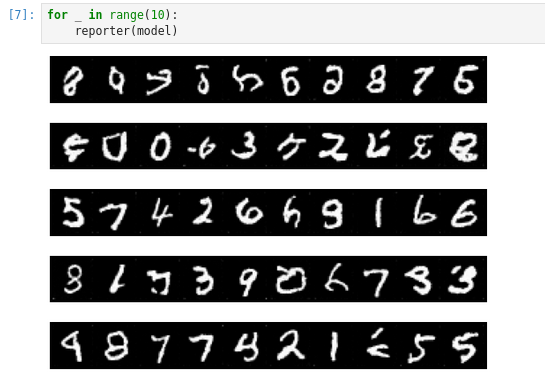
\includegraphics[width=0.7\textwidth]{./figures/ddpm_sampling.png}
  \caption{
    Sampling from a DDPM trained on the MNIST dataset.
  }
  \label{fig:week6:ddpm:sampling}
\end{figure}
